% METODOLOGÍA

\cleardoublepage

\chapter{Metodología}
\label{metodologia}

En este capítulo entraremos más en profundidad en los detalles técnicos y en las diferentes decisiones tomadas a lo largo del proyecto en cuanto a la descomposición del problema para adecuarlo al paradigma del aprendizaje por refuerzo.
\medskip

Comenzaremos hablando de los datos, cómo se obtuvieron y cómo los utilizaremos en nuestro proyecto y hablaremos de las diferentes piezas de este y los algoritmos escogidos para llevar a cabo los experimentos.
\medskip

\section{Obtención de los datos}
\label{obtencion-datos}

La toma de datos se hace mediante el análisis de archivos de vídeo tomados desde el propio dispositivo en un entorno controlado. Es importante destacar que la calidad de las imágenes no es alta, sobre todo en entornos en los cuales la iluminación no es favorable, por ejemplo en entornos con iluminación artificial. 
\medskip

\begin{figure}[H]
    \centering
	\subfloat[]{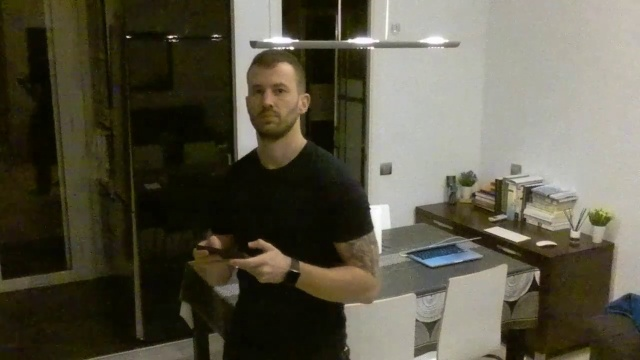
\includegraphics[width = 0.4\linewidth]{figuras/dataset/image2.jpg}}
	\hspace{0.05\linewidth}
	\subfloat[]{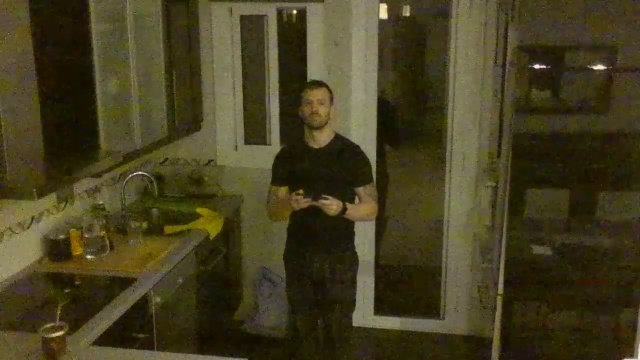
\includegraphics[width = 0.4\linewidth]{figuras/dataset/image7.jpg}}
	\hspace{0.05\linewidth}
	\subfloat[]{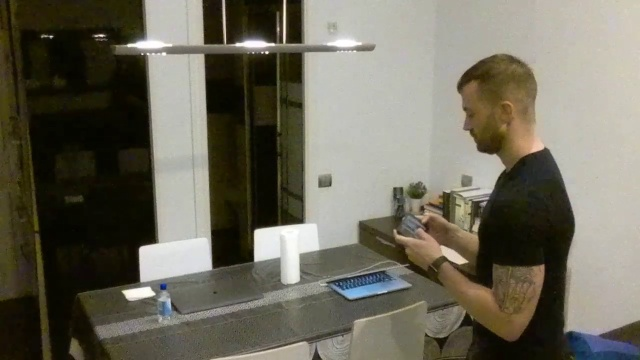
\includegraphics[width = 0.4\linewidth]{figuras/dataset/image8.jpg}}
	\hspace{0.05\linewidth}
	\subfloat[]{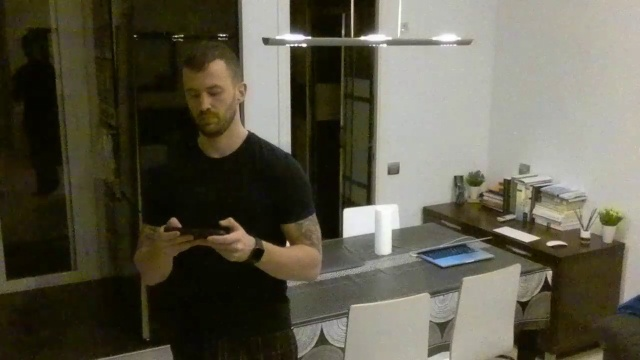
\includegraphics[width = 0.4\linewidth]{figuras/dataset/image1.jpg}}
    % \caption[Así aparece el rótulo en el índice]{Así aparece el rótulo en el texto.}
    \caption[Imágenes de ejemplo del conjunto final de datos]{Imágenes de ejemplo del conjunto final de datos.}
    \label{fig-dataset-imagenes-ejemplo}
\end{figure}
\medskip

El dispositivo nos proporciona una aplicación móvil para controlar la grabación y el almacenamiento de los videos que luego serán volcados en el ordenador para su posterior procesamiento, del cual hablaremos posteriormente.
\medskip


Se ha decidido también utilizar sólo imágenes procedentes del dispositivo y no incluir imágenes de terceras fuentes que podrían haber ayudado a mejorar el tamaño final de nuestro conjunto de datos ya que la idea es acercarse lo máximo posible a un entorno final real.
\medskip

Debido a las leyes vigentes sobre vuelo de drones, los escenarios en los cuales fueron grabados los videos se redujeron drásticamente a un entorno cerrado, lo cual nos lleva a pensar que más adelante podríamos tener un problema de overfitting en nuestro modelo.
\medskip

En un escenario ideal contaríamos con diferentes entornos que nos permitiesen descartar la posibilidad de que el agente aprenda que la posición de determinados objetos es condicionante para tomar una decisión y que se centrara solo en las persona de la imagen.
\medskip

\section{Preprocesamiento de los datos}
\label{preprocesamiento-datos}
\begin{figure}[ht!]
    \centering
    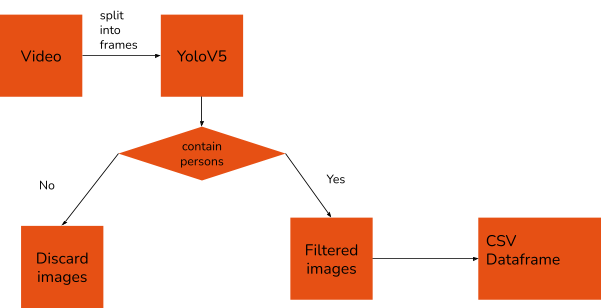
\includegraphics[scale=0.6]{figuras/data_preprocessing.png}
    % \caption[Así aparece el rótulo en el índice]{Así aparece el rótulo en el texto.}
    \caption[Pipeline del procesamiento del conjunto de datos]{Pipeline del procesamiento del conjunto de datos.}
    \label{fig-preprocesamiento-datos}
\end{figure}


Tras la recolección de videos y fotos desde el dispositivo, se realiza un primer proceso de filtrado. Este primer paso consiste en realizar un split de los archivos de video en frames individuales y realizar una operación de reducción del tamaño sobre los frames originales, pasando de 1280 píxeles de ancho y 720 píxeles de alto, a 640 píxeles de ancho y 360 píxeles de alto. Más adelante se tendrá que realizar una segunda reducción de las imágenes para adaptarlas al tamaño de entrada de la red convolucional previa al agente.
\medskip

Este primer paso de filtrado es posible gracias a los algoritmos de detección de objetos, mediante el uso de redes convolucionales neuronales, que nos proporcionan las coordenadas de las bounding box de aquellas clases de objetos que queremos encontrar en nuestro conjunto de datos.
\medskip

Durante el transcurso de nuestro proyecto utilizaremos \textit{YOLOv5}(\citep{youonlylookonce}), cuya implementación se encuentra disponible de forma gratuita como librería open source. Dicha implementación nos proporciona además múltiples configuraciones de la red. En nuestro caso, esto no fue muy relevante dado que solo lo utilizaríamos para una primera fase de preprocesamiento de las imágenes.
\medskip

Debido a que la red \textit{YOLOv5} fue entrenada sobre el conjunto de datos \textit{ImageNet} \citep{imagenet} para detectar 1000 clases de objetos diferentes, debemos modificarla para que sea capaz de detectar tan solo una persona en las imágenes que le pasamos, si es que la hay. La documentación de la librería nos ayuda a conseguir esto, de manera que tras una serie de pruebas tanto de diferentes arquitecturas de \textit{YOLO} como de configuración de los parámetros, en concreto: el intervalo de confianza y  el IoU threshold, la red nos devuelve la ubicación de la bounding box en donde se encuentra la persona si es que la hubiese.
\medskip

Sin embargo, para poder adaptar la salida de la red a nuestras necesidades, lo que hicimos fue calcular el punto central de la bounding box en coordenadas X e Y, para que nuestro agente intente acercarse a ese punto durante el entrenamiento en el menor número de pasos posible.
El resultado fue por un lado, un dataframe de Pandas que contenia la ruta de la imagen que \textit{YOLO} había filtrado y las coordenadas X e Y del punto central de la bounding box.
\medskip

Un punto a destacar es que las imágenes que no contenían personas fueron descartadas del conjunto de datos. Esta fue una decisión que se valoró al inicio con el fin de conseguir un agente y una definición más sencilla del problema. De no haber sido así, tendríamos que haber tenido en cuenta el hecho de que la imagen no presenta un punto objetivo y por lo tanto el dron debería permanecer quieto o girar hasta encontrar una persona.
\medskip

El número total de imágenes de nuestro conjunto de datos inicial tras este primer paso se reduce a tan solo 1690 imágenes. Sin embargo, y debido a que nuestro objetivo es modelar los movimientos de giro del dron tenemos que ser conscientes de cuántas imágenes contamos para que el dron nos detecte a la derecha, a la izquierda o en el centro de la imagen.
\medskip

En un primer análisis, nuestro conjunto de datos se encontraba completamente desbalanceado. Lo que hicimos para comprobar esto fue tomar las coordenadas centrales de la bounding box sobre el eje X que calculamos con \textit{YOLO} y comprobar en qué parte de la imagen se encontraba. Si esta coordenada se encontraba entre los píxeles 0 y 280, entonces el dron tendría que que girar a la izquierda, si se encontraba entre el 280 y el 360, entonces podríamos decir que el dron se mantendría prácticamente quieto, y si la coordenada se encontraba por encima de 360, el dron tendría que girar hacia la derecha.
\medskip

Los resultados de este análisis fueron los siguientes:

\begin{itemize}
    \item 340 imágenes se encontraban con la coordenada X en el lado izquierdo.
    \item 870 imágenes se encontraban con la coordenada X en el lado derecho.
    \item 480 imágenes se encontraban con la coordenada X en el centro de la imagen.
\end{itemize}

Debido a este desbalance, se tomó la decisión de igualar la cantidad de imágenes en cada lado, dejando un total de 340 imágenes por cada categoría, lo que hizo un total de 1020 imágenes finales para el entrenamiento y la validación de nuestro agente, lo que en contrapartida podría incrementar aún más el overfitting, pero nos aseguramos de que las decisiones que toma nuestro agente no se verán condicionadas por el número de acciones totales que debería tomar sobre un lado u otro. 
\medskip

Sin embargo, antes de tomar la decisión de descartar las imágenes se estudió la posibilidad también de realizar técnicas de data augmentation tal y como se recomienda en la literatura, utilizando técnicas de crop y volteo horizontal y vertical en cada una de las imágenes, pero la complejidad añadida de tener que recalcular el nuevo punto central hizo que descartemos esa posibilidad.
\medskip

Debido a que nuestro conjunto de datos no es muy grande, decidimos que el conjunto de entrenamiento sea el 90\%, del cual el 80\% se usará para la fase de entrenamiento de nuestro modelo y el otro 20\% se usará para la fase de test. El 10\% restante de nuestro conjunto, aproximadamente 100 imágenes, lo reservamos para la etapa de validación, de manera que probaremos los resultados de nuestro agente sobre un conjunto de imágenes que no haya visto previamente.



\section{Análisis de la solución e implementación}
\label{analisis-de-la-solucion-e-implementacion}

En la siguiente sección hablaremos de la implementación de cada uno de los elementos que componen nuestro problema, así como de las decisiones iniciales tomadas.
\subsection{Elección de los algoritmos utilizados por el agente}
\label{eleccion-de-algoritmos}

Para entrenar nuestro agente utilizaremos métodos que optimicen la \textit{policy} del agente, es decir, que optimicen la toma decisiones para maximizar la \textit{reward} del entorno.
\medskip

Comenzaremos utilizando el algoritmo \textit{REINFORCE Policy Gradient}, el cual se considera de los más sencillos dentro de la familia de \textit{Policy Gradient} y nos servirá como punto de partida para analizar los posibles problemas y limitaciones de nuestro entorno y nuestras definiciones. Con este algoritmo, el agente colecciona ejemplos del episodio utilizando para ello la \textit{policy} actual.
\medskip

\vspace{3ex}
\begin{algorithm}[H]
\label{algoritmo-reinforce-policy-gradient}
\SetAlgoLined
\medskip
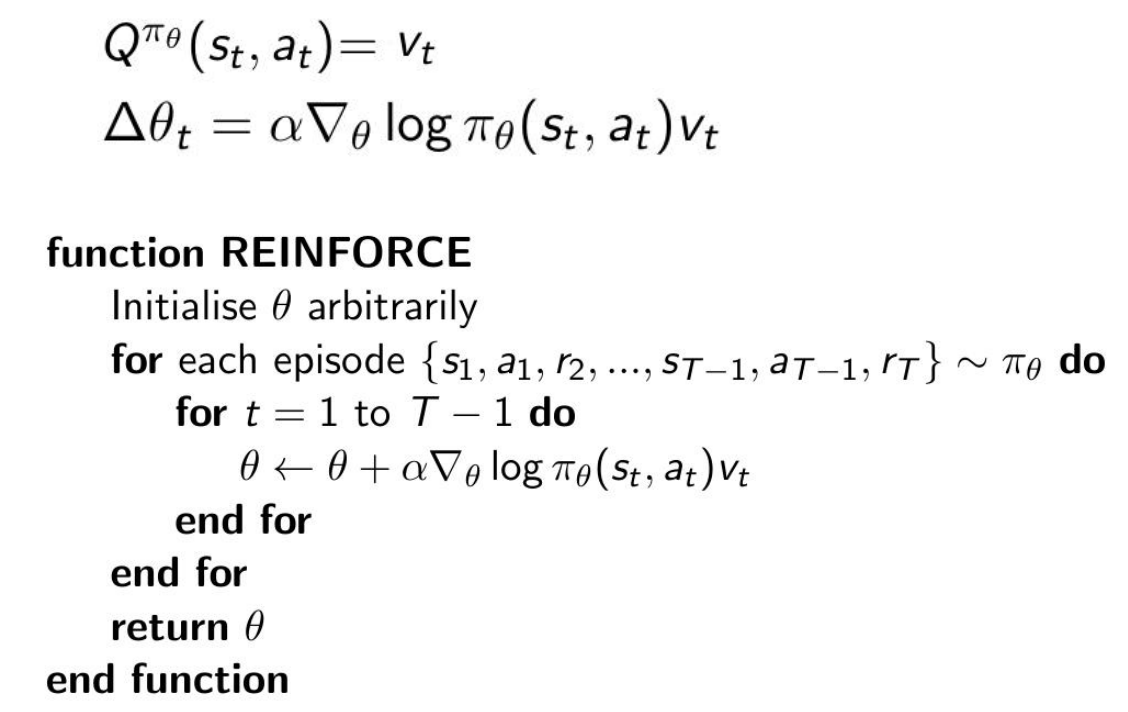
\includegraphics[width=0.7\textwidth]{figuras/reinforce_policy_gradient.png}
\caption{Algoritmo REINFORCE \textit{Policy Gradient}}
\end{algorithm}
\vspace{3ex}

	

Como siguiente paso, escogeremos nuevamente un algoritmo de la familia de \textit{policy gradient} para el entrenamiento del agente. En este caso, el algoritmo \textit{Actor-Critic} \citep{DBLP:journals/corr/abs-1801-01290}. La mayor diferencia entre este algoritmo y el anterior, es que en este caso contamos con 2 componentes separados: el \textit{Actor}, que será el responsable de devolver la distribución de probabilidades de cada una de las acciones del agente y el \textit{Critic}, que será el encargado d estimar el valor del estado en el que se encuentra dicho agente.
\medskip

\vspace{3ex}
\begin{algorithm}[ht!]
\label{alg-algoritmo-actor-critic}
\SetAlgoLined
\medskip
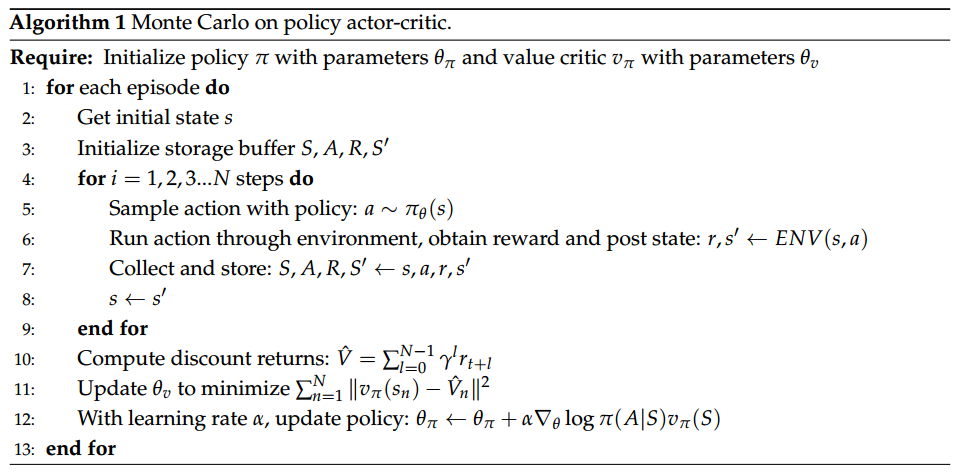
\includegraphics[width=0.8\textwidth]{figuras/algoritmo_actor_critic.png}
\caption{Algoritmo \textit{Actor Critic}}
\end{algorithm}
\vspace{3ex}

\subsection{Definición del estado}
\label{definicion-del-estado}

El estado es la representación del problema que el agente debe resolver. En este caso, el estado será una imagen de la cámara del dron, a la que se le aplicó previamente un procesamiento, tal y como comentamos en la sección \ref{preprocesamiento-datos}, junto con el punto en el que se encuentra el agente, expresado en un número entre 0 y 1, representando el 0 estar en el borde izquierdo de la imagen y 1 estar en el borde derecho de esta.
\medskip

Es decir, el agente recibirá un vector como entrada, de tamaño 4097. Los primeros 4096 elementos representan la imagen, la cual ha sido procesada por una \acrshort{cnn} preentrenada, que en nuestro caso ha sido VGG19 \citep{vgg19}, la cual recibe como entrada un vector de tamaño 224x224x3, es decir, una imagen en formato RGB de 224x224 píxeles. Si bien la elección de nuestra \acrshort{cnn} no fue basándonos en ningún criterio en particular, la idea era disminuir el tamaño de la entrada de nuestro agente. 
\medskip

También se tuvieron en cuenta diferentes soluciones para la definición del estado. Entre ellas, la posibilidad de que el estado se formase de varias imágenes al mismo tiempo, debido el componente temporal con el que cuenta nuestro problema. Este estado condicionaría también la arquitectura de la red de nuestro agente, dado que en este caso necesitaríamos tratar con redes recurrentes o en su defecto con redes de tipo Transformers \citep{transformers}, tal y como se explica en el trabajo realizado por \citet{luo2019end} y podemos ver en la figura \ref{fig-arquitectura-red-luo}, donde podemos ver que después del \textit{encoder}, tal y como se cita en el trabajo, se utiliza una red \acrshort{LSTM}.
\medskip

\begin{figure}[H]
    \centering
    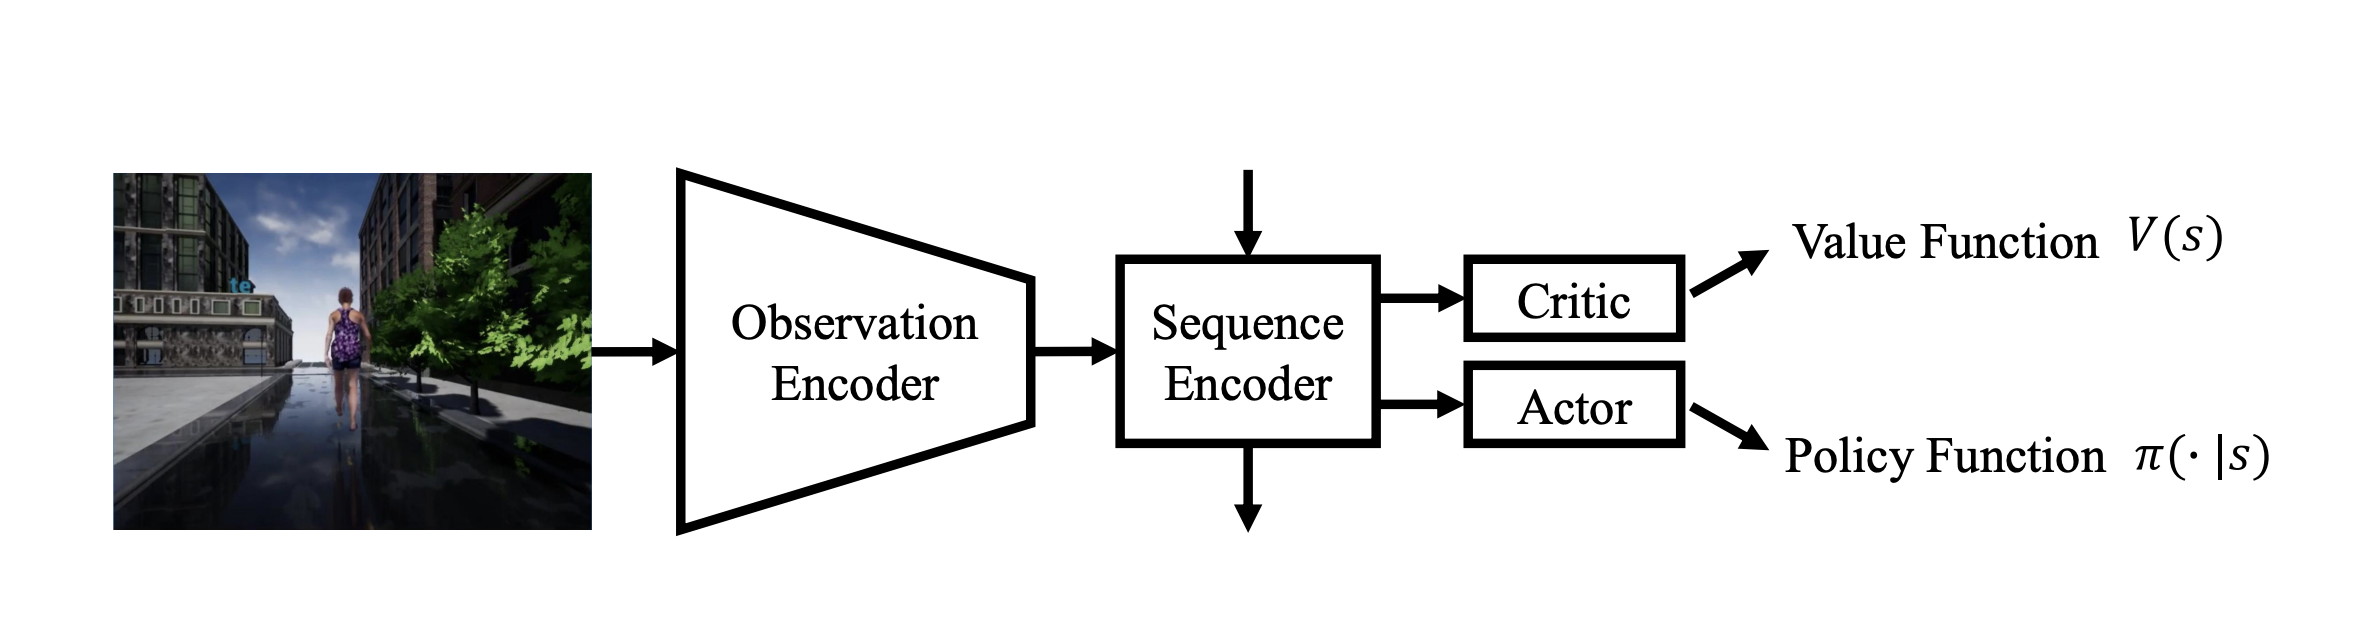
\includegraphics[scale=0.3]{figuras/luo_network_architecture.png}
    % \caption[Así aparece el rótulo en el índice]{Así aparece el rótulo en el texto.}
    \caption[Arquitectura de red propuesta por \citet{luo2019end}.]{Arquitectura de red propuesta por \citet{luo2019end}.}
    \label{fig-arquitectura-red-luo}
\end{figure}

Para aumentar la velocidad de nuestro entrenamiento, la imagen será preprocesada por la red convolucional al inicio de cada episodio y se mantendrá constante, dado que lo que iremos cambiando con cada acción durante el entrenamiento es el punto en el que se encuentra el agente.
\medskip

Por último, el estado contiene en su último elemento, el punto en el que se encuentra el agente en un momento dado, de manera que este debería ser capaz de tomar decisiones basándose no solo en la representación de la imagen sino también del valor que este valor tenga en ese instante.

\subsection{Definición de la recompensa}
\label{definicion-de-recompensa}

El desarrollo de la recompensa fue uno de los puntos críticos en cuanto a la implementación y la definición de nuestro problema. Por un lado, tenemos que intentar que nuestro agente sea capaz de ir aprendiendo los pasos intermedios que lleven a la obtención de la recompensa óptima, en el menor número de pasos posibles y por otro, definir cúanta recompensa en términos absolutos el agente recibirá cuando acaba correctamente el episodio, en contraposición a cuando llega al número máximo de intentos sin haber obtenido la recompensa máxima.
\medskip

La idea inicial fue crear una zona de recompensa proporcional a la distancia del punto en el que se encontraba el agente y el punto obtenido durante el preprocesamiento de los datos. Esto lo hicimos diviendo la imagen en secciones longitudinales de tamaño fijo. Dado que nuestra imagen era de 640 píxeles de ancho, lo que hicimos fue dividirla en 32 secciones de 20 píxeles cada una. La recompensa final obtenida sería inversamente proporcional a la distancia, medida en número de secciones, en que el agente se encontraba con respecto al punto objetivo. De manera que si el agente se encontraba a 5 secciones de nuestro punto final, obtendría menos recompensa que si se encontrara a 2 secciones, tal y como se puede observar en el algoritmo \ref{algrecompensainicial}:
\medskip
\vspace{3ex}
\begin{algorithm}[H]
\label{algrecompensainicial}
\SetAlgoLined
\medskip
\begin{enumerate}
	\item Dividimos la imagen en secciones longitudinales de tamaño fijo $Secciones_{total}$.
	\item Establecemos una recompensa máxima del entorno $Recompensa_{max}$.
	\item Calculamos la sección en la que se encuentra nuestro agente:
	$Seccion_{agente} = round(Pagente_{pixels} / Ancho_{imagen})$.
	\item Calculamos la sección en la que se encuentra nuestro punto final:
	$Seccion_{objetivo} = round(Pobjetivo_{pixels} / Ancho_{imagen})$.
	\item Si $Seccion_{agente} = Seccion_{objetivo}$ devolvemos $Recompensa_{max}$.
	
	Sino devolvemos $1 - (Seccion_{agente}-Seccion_{objetivo}/Secciones_{total}) $
\end{enumerate}
	\caption{Algoritmo de recompensa inicial}
\end{algorithm}
	
\vspace{3ex}

Lo que conseguimos con esta recompensa fue obtener un \textit{heatmap} alrededor del punto objetivo, de manera que el agente podría interpretar si se estaba acercando o alejando. 
\medskip

La recompensa máxima fue establecida a 1, de manera que los saltos entre las recompensas parciales y la recompensa final fuese siempre proporcional a la distancia. Más adelante también comprobaremos cómo este valor puede afectar al desarrollo de una solución por parte de nuestro agente.
\medskip

\begin{figure}[H]
	\centering
	\parbox{5in}{
		\centering
		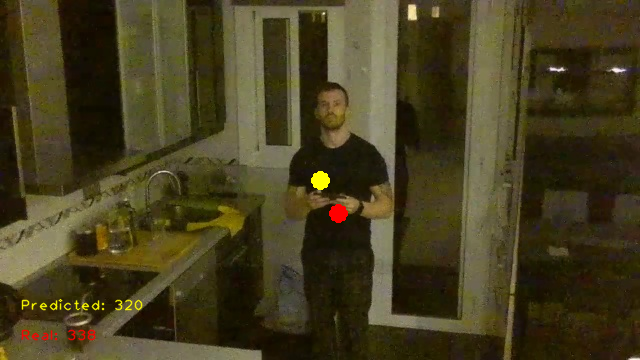
\includegraphics[scale=0.35]{figuras/recompensa/recompensa_maxima.png}
	}
	\qquad
	\begin{minipage}{5in}
		\centering
		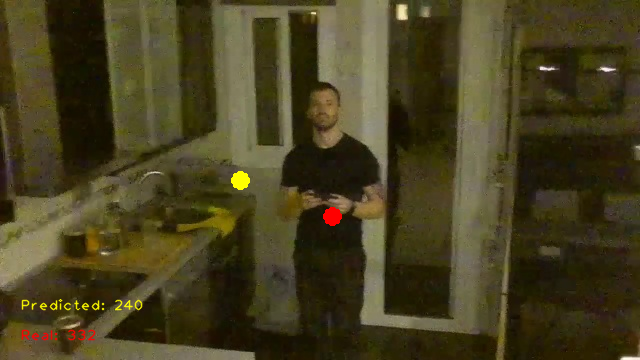
\includegraphics[scale=0.35]{figuras/recompensa/recompensa_no_maxima.png}
	\end{minipage}
	\caption[Comparación de recompensa sobre la misma imagen dados dos puntos de vista distinto.]{La misma imagen, con 2 puntos definidos por el agente a diferente distancia del punto objetivo. La imagen superior obtendría la puntuación máxima mientras que la imagen inferior solo obtendría una recompensa relativa a la distancia del punto objetivo.}%
	\label{fig-recompensa-imagenes}
\end{figure}


En la figura \ref{fig-recompensa-imagenes} podemos observar cómo funciona nuestro sistema de recompensa inicial. En la imagen situada en la parte superior, el punto amarillo, que representa el punto en el que se encuentra el agente, está dentro de la misma sección que el punto objetivo, y por lo tanto la recompensa será máxima. Mientras que en el caso de la imagen inferior, el punto donde se encuentra el agente está a una distancia mayor a una sección (definida por defecto en 20 píxeles), y por lo tanto la recompensa será proporcional al número de secciones que se encuentra hasta llegar al punto objetivo.

\subsection{Definición del entorno}
\label{definicion-del-entorno}

Para desarrollar el entorno, lo que se hizo fue implementarlo siguiendo como ejemplo los entornos propuestos por OpenAI Gym \citep{openaigym}. Esto nos facilitó tener una primera estructura y una primera definición de los métodos que deberíamos implementar.
\medskip

Al inicio de cada episodio, nuestro entorno se encargará de devolver una imagen del conjunto de datos (entrenamiento, test o validación), así como las coordenadas del punto en el que se encuentra la persona, expresados en píxeles, que es lo que compone nuestro estado tal y como describimos en la sección \ref{definicion-del-estado}. Estos valores se guardan durante toda la ejecución del episodio y se renuevan una vez que se empieza uno nuevo.
\medskip


La ejecución de cada acción sobre el entorno nos devolverá un nuevo estado, la recompensa asociada con ese estado y un valor que nos indicará si el estado es final o no, es decir, si el episodio finaliza en ese estado. 
\medskip

El algoritmo \ref{environment-step-action} detalla el pseudocódigo utilizado tras recibir una acción por parte del agente. Podemos observar que este algoritmo mueve el punto del agente basándose en la acción que este toma, siempre en una cantidad fija de píxeles, que corresponde con el tamaño de cada una de las secciones en las que fue dividida la imagen tal y como se explica en el apartado \ref{definicion-de-recompensa}. Esto se hizo de tal forma que el agente se moviese siempre a una sección diferente y por lo tanto la recompensa obtenida también sea diferente.
\medskip

\vspace{3ex}
\begin{algorithm}[H]
	\label{environment-step-action}
	\SetAlgoLined
	\medskip
	$width \gets 640$

	$distance \gets 20$

	\If{accion == 'LEFT'}{
		$point \gets point - distance$
	}
	\If{action == 'RIGHT'}{	
		$point \gets point + distance$
	}
	$point \gets torch.clamp(point, 1, width-1)$

	$reward \gets calculateReward(point)$

	$done = EnvironmentMaxReward == reward$

	\Return{reward, point, done}
	\caption{Ejecutar acción en el entorno}
\end{algorithm}
\vspace{3ex}

Podemos observar también que la acción de permanecer quieto no tiene ninguna consecuencia en el estado del agente y la utilizaremos como posible acción para finalizar el episodio por parte del agente.
\medskip

Durante las fases de entrenamiento, testeo y validación de nuestro agente, cada una de las acciones sobre el entorno involucra el cálculo de la nueva posición del punto en el que se encuentra el agente. Una vez el agente fuese desplegado para controlar el dron, cada ejecución de la acción involucraría la ejecución de esa acción en el dron, ya sea girar a la derecha, a la izquierda, o permanecer quieto y obtener una nueva imagen. En este caso, el punto de vista del dron siempre sería el centro de la imagen.
\medskip

\subsection{Definición del agente}
\label{definicion-del-agente}

El agente es el componente de nuestra solución que se encarga de interactuar con el entorno. En este caso, el agente será el encargado de tomar la decisión de girar la cámara del dron a la izquierda, a la derecha o de permanecer quieto, dado un estado del entorno, el cual está definido como se detalla en la sección \ref{definicion-del-estado}.
\medskip

\begin{figure}[H]
    \centering
    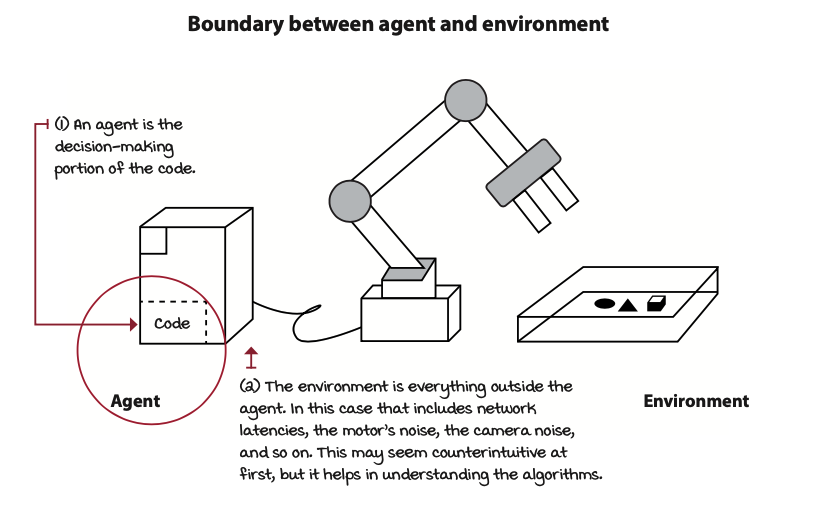
\includegraphics[width=1\textwidth]{figuras/agent_responsabilities.png}
    % \caption[Así aparece el rótulo en el índice]{Así aparece el rótulo en el texto.}
    \caption[Interacción agente-entorno.]{Interacción agente-entorno. Imagen tomada del libro \textit{Grokking Deep Reinforcement Learning} \citet{grokkingreinforcementlearning}.}
    \label{fig-agent-picture}
\end{figure}

El objetivo de nuestro agente será encontrar aquellas acciones que maximicen las recompensas obtenidas. Este objetivo será alcanzado dependiendo del algoritmo que utilicemos para ello, pero independientemente de esto, las recompensas obtenidas y el conjunto de acciones será el mismo.
\medskip

En cuanto a la implementación, el agente será una red neuronal cuya arquitectura iremos variando según los diferentes experimentos, que extenderá de la clase \textit{nn.Module} de \textit{PyTorch} y a la cual le añadiremos métodos propios para facilitar la lectura del código.


\subsection{Entrenamiento}
\label{entrenamiento}

En cuanto al proceso de entrenamiento, destacamos el hecho de que cada episodio está compuesto por una sola imagen. Es decir, cuando el agente llegue a la recompensa máxima establecida en cada imagen o cuando se llegue al número máximo de acciones que definimos durante el bucle de ejecución, el episodio acabaría. 
\medskip

La inclusión de un número máximo de pasos por imagen fue una decisión tomada para que nuestro agente no entrase en un bucle infinito si decidiese por ejemplo, girar siempre hacia la derecha, llegando al extremo de la imagen donde no se encuentra la persona. Esta decisión también nos lleva a experimentar con un parámetro extra en nuestro entrenamiento, ya que un número muy elevado de acciones puede llevarnos a que el agente no aprenda correctamente y por lo tanto la exploración sobre el entorno no tenga ningún efecto, y por otro lado, un número muy pequeño podría llevarnos a que el agente no tuviese el tiempo suficiente para aprender la policy adecuada dado el estado. Por lo general, este valor oscilaba entre 50 y 100 acciones por imagen, aunque también se realizaron pruebas con valores menores y mayores a estos.
\medskip

Debido al problema de la falta de imágenes en diferentes entornos, tal y como comentamos en la sección \ref{preprocesamiento-datos}. Se tomó la decisión de que el punto inicial se inicialice de manera aleatoria, entre un valor de 0 y 1, que luego será multiplicado por el ancho de la imagen para darnos las coordenadas reales y calcular la recompensa en ese punto. La idea detrás de esta decisión es dotar al entrenamiento de un componente aleatorio y por lo tanto evitar que nuestro agente pueda realizar overfitting sobre el conjunto de datos, dado que para una misma imagen , durante el entrenamiento, el punto de partida sea diferente.
\medskip

Durante el proceso de entrenamiento se realizaron multitud de pruebas, no solo en lo que respecta a los parámetros de nuestro modelo, sino también a los criterios de parada de cada episodio, el número máximo de acciones a tomar o la recompensa obtenida al seleccionar la acción de permanecer quieto. De estas diferentes decisiones hablaremos en cada uno de los experimentos.
\medskip

\subsection{Evaluación}
\label{evaluacion}

Para evaluar la calidad de los resultados del agente, comprobaremos sobre cada imágen del conjunto de validación, cuándo el agente decide quedarse quieto y la recompensa que obtiene al hacerlo. Esto se asemeja al comportamiento real que tendría al ser desplegado en el dron.
\medskip

La evaluación comienza con las coordenadas del punto del agente en las coordenadas centrales de la imagen, de manera que simula el punto central de la cámara del dron. Lo que se hace a continuación es ejecutar el agente sobre ese estado y aplicar las acciones de este hasta encontrarnos con la acción de permanecer quieto, lo cual sería el indicador de que el agente se encuentra en la posición en la que se encuentra la persona. En ese momento, dado que contamos con las coordenadas reales obtenidas durante el procesamiento, calculamos la recompensa.
\medskip

Esta operación se realiza tanto para el conjunto de test durante el entrenamiento, como para el conjunto de validación después del entrenamiento. En ambos casos, nuestro modelo funciona en modo evaluación y por lo tanto no se propagan cambios a los pesos de este.
\medskip

Además de la recompensa total, nos interesa en este caso obtener un agente que decida moverse de manera uniforme hacia una dirección en el menor número de acciones posible. Pensemos que cada acción que tome el agente será una acción que el dispositivo tendrá que realizar y por lo tanto es tiempo de ejecución que se pierde. Es decir, un agente que consigue la recompensa máxima en 5 acciones será más valioso que uno que la consiga en 10.
\medskip

Aunque el hecho de conseguir la recompensa máxima del entorno en nuestro caso no es indicativo de la calidad de nuestro agente, por ejemplo podemos pensar que nuestro agente se acerca al punto en el que se encuentra la persona, sin llegar a estar exactamente en donde debería, pero sin embargo lo hace de manera consistente, en un número de acciones reducido por frame, lo que al final nos permite ser más rápidos en la ejecución final y por lo tanto, a efectos prácticos, nos puede incluso llegar a ser más valioso.
\medskip

\begin{figure}[ht!]
	\centering
	\subfloat[Ubicación del agente tras 2 acciones]{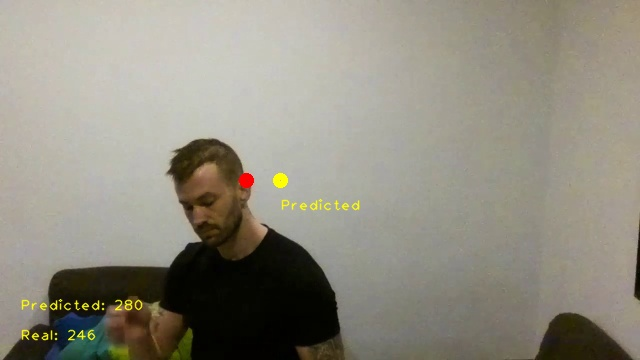
\includegraphics[width = 0.47\linewidth]{figuras/recompensa/comparacion_2_acciones_tomadas.jpg}}
	\hspace{0.05\textwidth}
	\subfloat[Ubicación del agente tras 6 acciones]{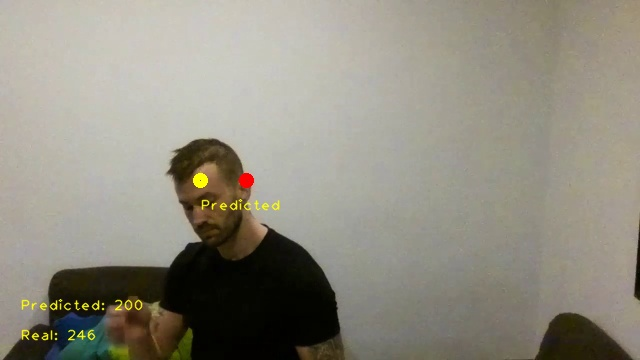
\includegraphics[width = 0.47\linewidth]{figuras/recompensa/comparacion_6_acciones_tomadas.jpg}} 
	\caption[Imagen ejecutada en dos experimentos distintos, a la misma distancia del punto objetivo, con diferente número de acciones.]{Imagen ejecutada en dos experimentos distintos, cuyo punto predicho se encuentra a la misma distancia del punto objetivo, con diferente número de acciones.}%
	\label{fig-comparacion-numero-de-acciones}
  \end{figure}
\medskip

Un ejemplo de este comportamiento lo vemos en la figura \ref{fig-comparacion-numero-de-acciones}, en el que se puede ver que sobre la misma imagen, ejecutada en 2 experimentos diferentes, tenemos 2 puntos de vista por parte del agente a prácticamente la misma distancia. La imagen de la izquierda requirió de solamente 2 acciones, mientras que la imagen de la derecha de 6 acciones. Por lo tanto, para esta imagen nos interesaría el agente que produjo la imagen de la izquierda.
\medskip

Debido a la alta latencia que se producia al conectar el dron con nuestro ordenador, la ejecución en el dispositivo real no fue posible. Lo que se hizo en su lugar fue analizar frame por frame una serie de videos grabados desde el dispositivo, ejecutabdi una acción en cada uno de ellos para que simulara la acción a tiempo real que tomaría el agente.
Todos estos factores están sujetos a una evaluación subjetiva que iremos comentando más adelante en los diferentes experimentos que realicemos.